\chapter{架设PT网站所需要的技术综述}

\section{BitTorrent协议, Bencode编码与Torrent文件}
\label{sec:BitorrentProtocol}

BitTorrent协议\footnote{完整协议内容见参考文献: BEP-0003\cite{bramcohen2008bep0003}}(以下简称BT)是用在对等网络中目标为用户群对用户群(Peer-to-peer)的文件分享网络协议, 最大的特点为下载同一文件的用户越多, 下载该文件就越迅速。下载如果不关闭相应的BT客户端软件的话, 继续维持上传状态, 就可以该形式``分享''所下载的文件, 在这种场景下, 每一个BT客户端都起到类似CDN(Content Delivery Network, 内容分发网络)的作用。

BT协议将所需要分享的单个文件或者一组文件按照用户指定的顺序平铺成连续的总和二进制数据段, 然后按照用户指定的分块大小(Trunk size)进行补齐与分块, 使用SHA-1算法逐分块地对二进制数据段进行哈希, 生成相应分块的哈希值, 各分块的哈希值简单按先后顺序前后拼接在一起, 成为总和二进制数据段的哈希值, 这个总和哈希值在之后的使用中起到校验所下载的文件的作用。

由于上述平铺总和式的校验方式, 必须要对之后所下载的数据按照原始文件长度进行切割方可得到原始语义上的文件。同时, 为了方便地将这些分块校验码信息、文件长度信息在互联网上传播, 需要一种文件格式将上述信息进行编码。BT协议的提出者Bram Cohen创造性地提出了Bencode编码规则, 并在之后的Torrent文件(以下称作种子文件)生成步骤中进行了相应的实现。

Bencode编码的种子文件使用ASCII字符进行编码, 使得即使在普通文本编辑器中打开也能读懂其中的语义。Bencode中定义了字符串(Byte strings)、整数(Integers)、线性表(Lists)以及字典(Dictionary, 即关联数组(associative arrays))四种基本数据类型, 其中线性表类似于能存储任意数据结构类型的数组, 字典类似于键值对, 通过他们的组合就可以得到足够复杂的层级结构。

Bencode编码将要编码的内容通过简单的字母对括起来\cite{wikieditors2019bencode}, 或者是指定长度后用冒号表示出来。如整数用i和e括起来, `i233e`表示正整数233, `i-233e`表示负整数-233。字符串则是``长度:内容'', 如`12:aixiefuwoaix`表示``aixiefuwoaix''这个字符串。线性表允许不同的数据类型混杂, 使用l和e括起来, 比如对前述的两种数据结构, `l12:aixiefuwoaixi\-233ee'表示依次的字符串``aixiefuwoaix''以及正整数233。字典则将要编码的内容用d和e括住, 每一项的键和值必须首尾相接, 且键只能为字符串类型, 不能是整数, 排序上, 按照字典序排列键的字符串。如键为``aixiefuwoaix''值为正整数233, 紧接键为``nukkayg''值为负整数-233的字典表将被编码为`d7:nukkaygi-233e12:aixiefuwoaixi233ee'。

那么Torrent种子文件的结构也就呼之欲出了。根是一个字典, 下有一个键为``info''的字典节点, info字典的第一个键值对键为``files'', 值为线性表, 线性表中的各个节点又以字典和线性表的形式存放着所分享的不同文件的具体长度。info字典的第二个键值对键为``name''值为所分享的文件文件名, 或是文件夹名。info字典的第三个键值对键为``piece length'', 表示用户指定的分块大小长度, 值是正整数, 通常是2的幂次。紧跟着的info字典的第四个键值对键是``pieces'', 值就是前述的总和哈希值, 以字符串的形式存储。

\begin{figure}[ht!]
	\centering
	\begin{subfigure}{0.45\textwidth}
		\centering
		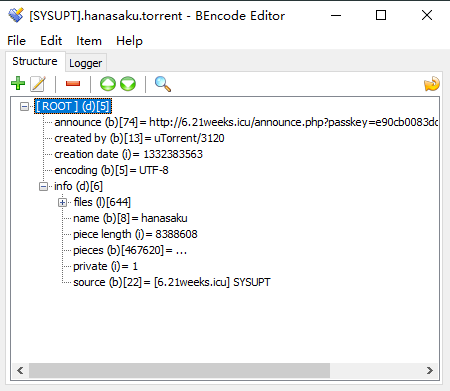
\includegraphics[width=\textwidth]{support-files/2.1-torrent-file-in-bencode-editor.png}
		\caption{在Bencode Editor中打开}
		\label{fig:torrent_in_bencode}
	\end{subfigure}
	\makebox[0.05\textwidth]{}
	\begin{subfigure}{0.45\textwidth}
		\centering
		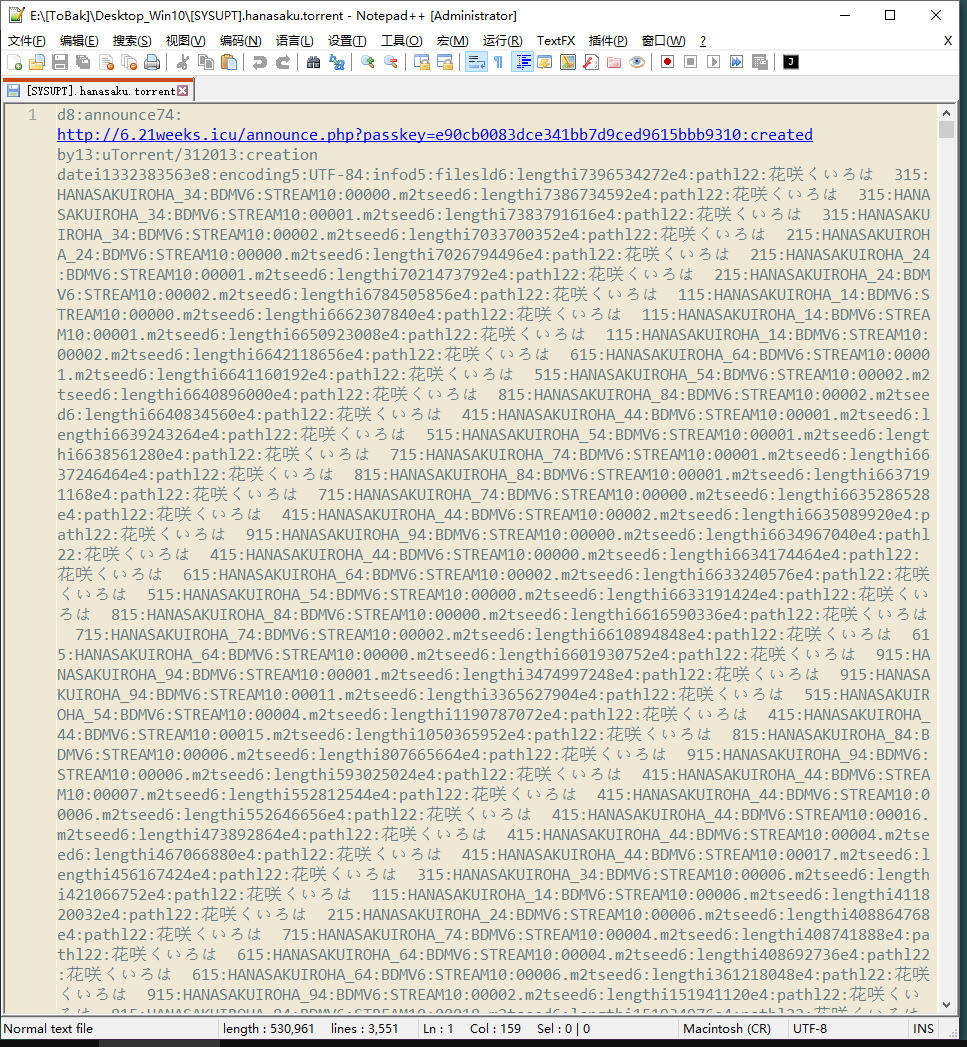
\includegraphics[width=\textwidth]{support-files/2.1-torrent-file-in-text-editor.png} 
		\caption{在文本编辑器中打开}
		\label{fig:torrent_in_text_editor}
	\end{subfigure}
	\caption{torrent文件}
	\label{fig:torrent}
\end{figure}

将这样构成的一个种子文件通过互联网分享出去, 得到该文件的人相当于得到了一份完整的文件校验信息。将这个文件交给BT客户端软件进行解析。通常在前述的``info''节点之前还会有一个``announce-list''节点, 记录后文中将要提到的Tracker服务器的地址信息。BT客户端得到Tracker列表后, 和Tracker服务器进行通信, 取得对等方列表(Peer list), 也就是网络上正在上传/下载这份种子文件所描述的资源的BT客户端的IP地址及端口号信息。通信内容也是用Bencode方式进行编码的, 下层协议一般是http或https。得到对等方BT客户端的IP地址及端口号后, BT客户端之间就可以发起进一步的通信, 进行实际的文件内容传输。其中囊括拥塞控制等算法在内的具体传输协议既可以使用原始BT协议中定义的一套基于TCP的协议, 也可以替换成BEP-0029\cite{arvidnorberg2009bep0029}(BitTorrent Enhancement Proposals No.29)中提出的基于UDP的μTP协议, 具体算法步骤参见附录中的链接, 在此不再赘述。


\section{适用于BT协议的Tracker服务器及Private Tracker}
\label{sec:TrackerAndPrivateTracker}

事实上, 一个BT发布平台本身也必须实现一个Tracker。Tracker负责记录每一个正在上传/下载相应种子文件所代表的资源的对等方(以下记作Peer)的BT客户端的IP地址和端口。也就是说, 一个Tracker必须维护这样一个表, 主键是种子文件的特征值, 字段包括该正在上传/下载该主键所代表的种子文件的Peer信息, 也即前述的地址和端口。在具体的实现中, 上面提到的这个特征值实际上会用前述info字典整体的长40字符的SHA-1哈希值来表示, 这也是著名的衍生于BT协议的magnet磁力链地址\cite{greghazel2008bep0009}的核心所在, 因与本文不直接相关, 此处按下不表。

BT客户端和Tracker发起通信(以下记作announce), BT客户端将自己正在上传/下载的种子的特征值(peer\_id)、BT客户端在两次announce之间对该种子的上传/下载量(uploaded/downloaded)等信息通过HTTP GET请求参数的方式向Tracker传送。Tracker则通过Bencode编码的方式, 将BT客户端所需要的peer\_id对应的对等方列表(peers), peers是一个List, 每个项里面又用Dictionary的形式记录着peer\_id(种子特征值), ip(对等方的IP 地址)以及port(对等方BT客户端监听的端口号)。有了这些信息, 一方BT客户端就可以向对等方BT客户端发起通信。


\section{BT客户端软件}

BT协议提出之初, 作者Bram Cohen就实现了一版BT客户端软件`BitTorrent'\footnote{\url{https://www.bittorrent.com/downloads}}, 随后他加入了商业公司`BitTorrent, Inc.'\footnote{\url{https://www.bittorrent.com/}}。所以BitTorrent既是协议的名称, 也是BT协议客户端软件的名称, 同时还是目前负责开发维护BT协议的商业公司的名称。

BT客户端就是直接面对用户的BT协议UI, 目前常见的BT客户端有uTorrent\footnote{\url{https://www.utorrent.com/}}, qBittorrent\footnote{\url{https://www.qbittorrent.org/}}等, 其中前者为BitTorrent, Inc.公司开发的商业共享软件, 可以免费下载使用; 后者是开源软件, 基于libtorrent-rasterbar\footnote{\url{https://www.libtorrent.org/}}这一开源BT协议的实现。

BT客户端的工作主要分为以下几步:

\begin{enumerate}[label=(\arabic*),leftmargin=*]
\item 监听指定端口, 以接受 \ref{enum:connect} 中将要描述的来自对等方BT客户端的传入连接。

\item 解析用户输入的Torrent文件, 取得种子特征值、Tracker服务器列表等关键信息。

\item 根据特征值和Tracker服务器的域名/IP地址, 向Tracker发起HTTP GET请求, GET的请求参数以及返回的结果如\ref{sec:TrackerAndPrivateTracker}中所述。

\item \label{enum:connect}根据返回的peers(对等方列表)中的IP地址和端口号, 向对等方的BT客户端发起连接。

\item \label{enum:transfer} \ref{enum:connect}中的连接建立后, 开始逐分块的二进制数据传送。可以是传统的TCP, 也可以是μTP。

\item 得到完整的一段分块的数据后, 根据\ref{sec:BitorrentProtocol}中所述的各分块SHA-1校验码进行校验。如果校验通过, 则放入缓存, 等待写入磁盘。如果校验出错, 则丢弃该分块。\textbf{通过这样分块验证/传送的机制, 可以最大限度保证数据损坏局限在小范围内, 体现了传输协议的高可用性}
。

\item \label{enum:write}将一定数量的已完成分块写入磁盘。

\item 重复 \ref{enum:transfer} \~{} \ref{enum:write} 中的步骤, 直至种子文件里描述的所有分块都写入磁盘。
\end{enumerate}




\section{Laravel MVC框架}
\label{sec:Larvel}

Laravel\footnote{\url{https://laravel.com/}}是美国开发者Taylor Otwell于2011年6月发布初版的用PHP编写的开源MVC框架。它的代码组织清晰, 并且使用了新生代PHP强大的扩展包(Composer)包管理机制, 使之成为一个非常现代化的Web应用开发框架。

Laravel根据模块组织文件结构\footnote{\url{https://laravel.com/docs/7.x/structure}}。项目的/app/Models目录下存放着项目所定义的数据结构模型(Model); /app/Http/Controller目录下存放着大多数开发所需要的后端逻辑, 即控制器(Controller)部分; /resources/views下存放着项目要向用户展现的视图(View)模板。

由于PHP的语法继承自C语言系列, 加上目录结构清晰、有完善的包管理机制, 使得接下来的开发非常高效。


\section{UNIT3D-Community-Edition}

UNIT3D-Community-Edition\footnote{\url{https://github.com/HDInnovations/UNIT3D-Community-Edition}}(以下简记作UNIT3D)是笔者选用的二次开发原型。他由美国开发者HDVinnie发起创建, 目前最新版本是v2.3.0。

UNIT3D的文件结构如\ref{sec:Larvel}中所述。其具有较好的UI, 同时作为种子发布平台的功能基本完善。但是, 由于作者是业余开发该项目, 加上测试人员并不多, 部分功能只是打桩而尚未实现, 而且有些使用习惯与国内用户并不相同。因此, 为了更好地将其投入使用, 笔者及同好们进行了大量的测试、调研, 并确定了二次开发的方向及计划。







% \label{cha:example}
% \section{图像的插入}
% \subsection{镶嵌在文中的图像}
% \label{sec:Images}
% \begin{wrapfigure}{r}{0.5\linewidth}
% 	\centering
% 	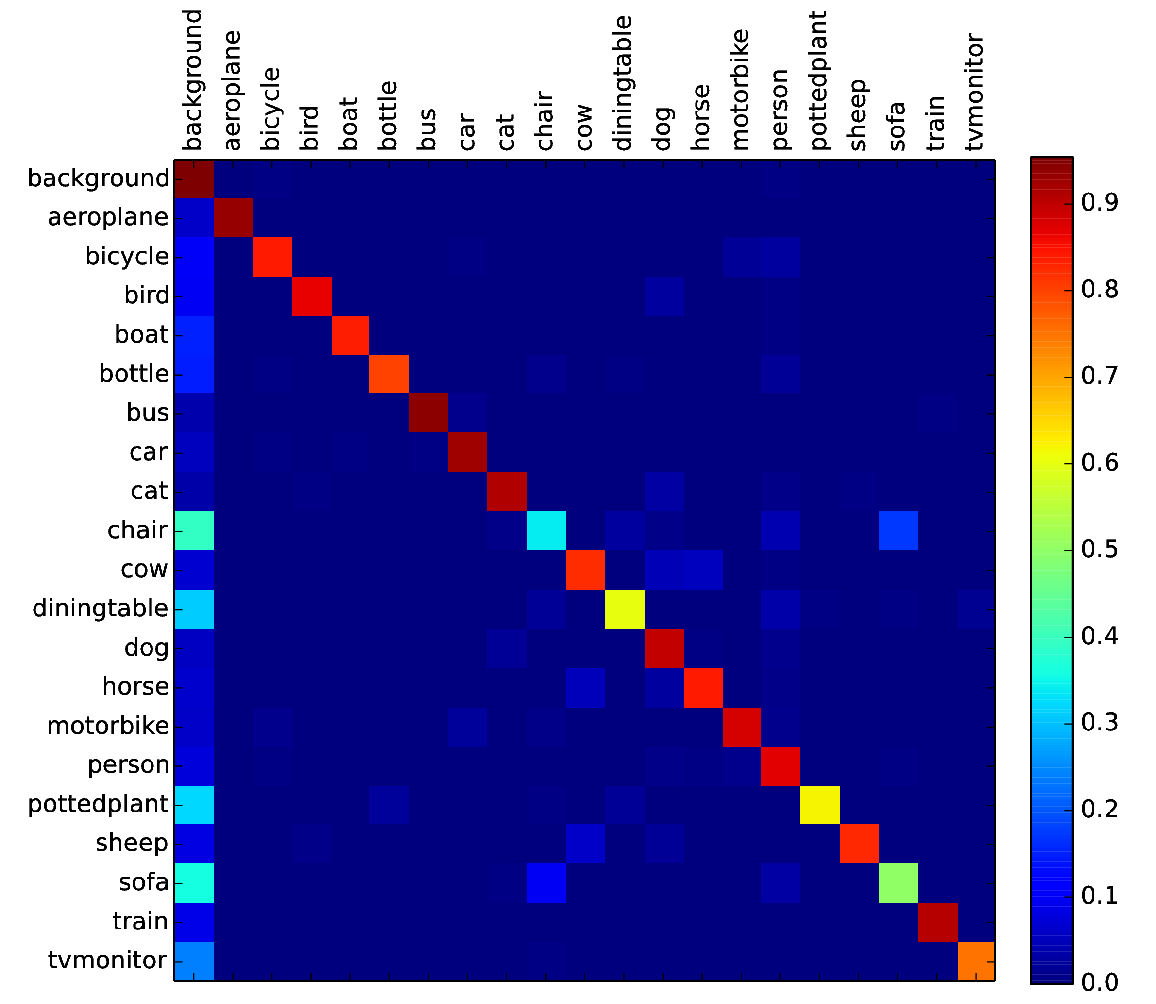
\includegraphics[width=0.5\textwidth]{image/result/confusion.pdf}
% 	\caption{镶嵌在文中的图像}
% 	\label{fig:confusion}
% \end{wrapfigure}
% 论文主体是毕业论文的主要部分,必须言之成理,论据可靠,严格遵循本学科国际通行的学术规范。在写作上要注意结构合理、层次分明、重点突出,章节标题、公式图表符号必须规范统一。论文主体的内容根据不同学科有不同的特点,一般应包括以下几个方面: (1)毕业论文(设计)总体方案或选题的论证; (2)毕业论文(设计)各部分的设计实现,包括实验数据的获取、数据可行性及有效性的处理与分析、各部分的设计计算等; (3)对研究内容及成果的客观阐述,包括理论依据、创新见解、创造性成果及其改进与实际应用价值等; (4)论文主体的所有数据必须真实可靠,凡引用他人观点、方案、资料、数据等,无论曾否发表,无论是纸质或电子版,均应详加注释。自然科学论文应推理正确、结论清晰;人文和社会学科的论文应把握论点正确、论证充分、论据可靠,恰当运用系统分析和比较研究的方法进行模型或方案设计,注重实证研究和案例分析,根据分析结果提出建议和改进措施等。
% \subsection{单张图像的插入}
% \begin{figure}[h]
	\centering
	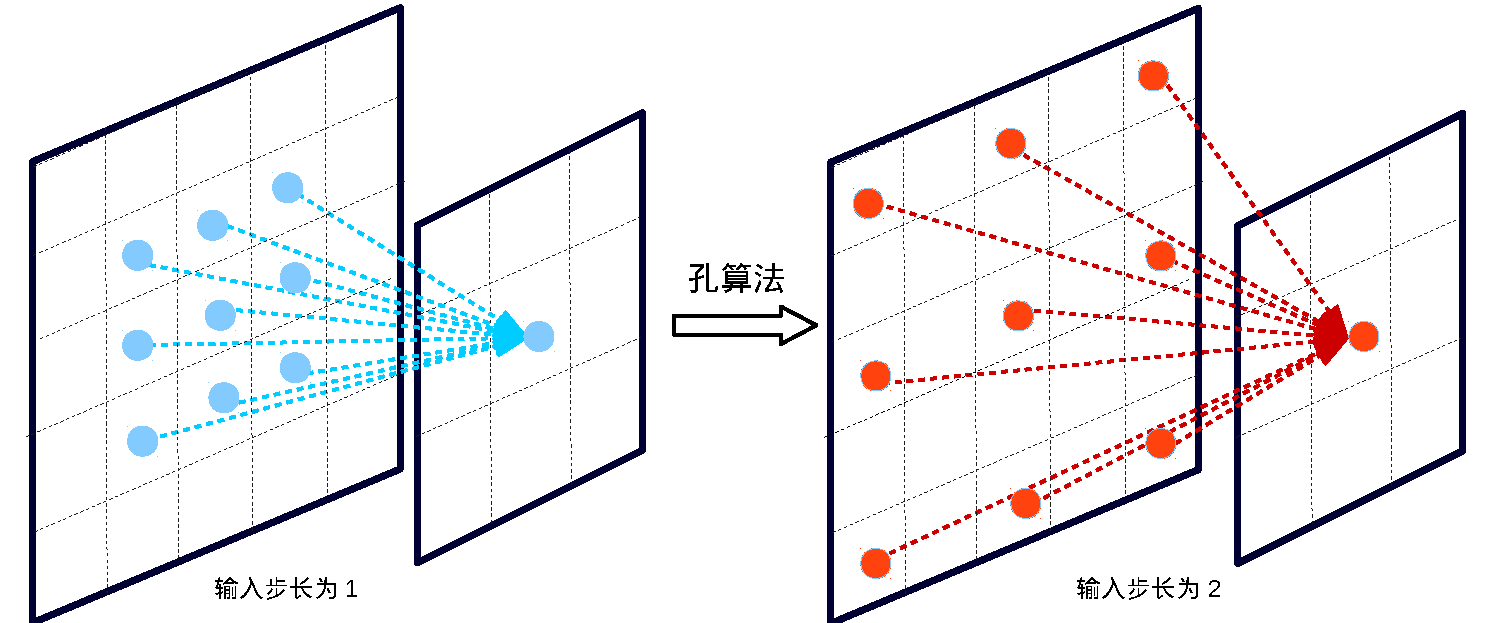
\includegraphics[width=0.5\textwidth]{image/illustration/hole.pdf}
	\caption{单张图像}
 	\label{fig:hole}
\end{figure}


% \subsection{多张图像的并排插入}
% \label{sub:多张图像的并排插入}
% \begin{figure}[h!]%文中的Grid-LSTM模型做的语义图像分割的例子
	\centering
	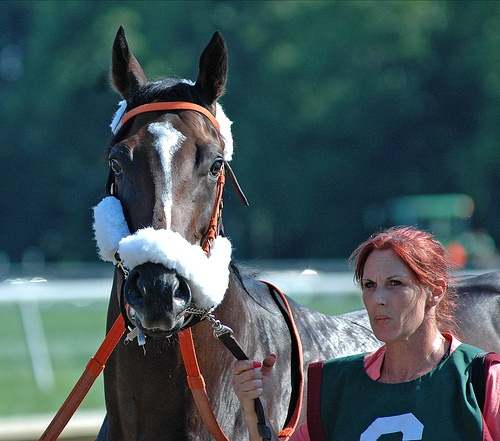
\includegraphics[width=.2\textwidth,height=.15\textwidth]{image/example/2007_000799.jpg}
	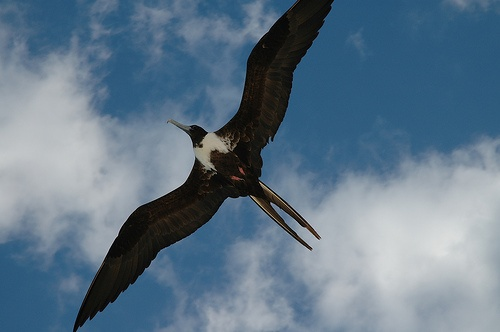
\includegraphics[width=.2\textwidth,height=.15\textwidth]{image/example/2007_002094.jpg}
	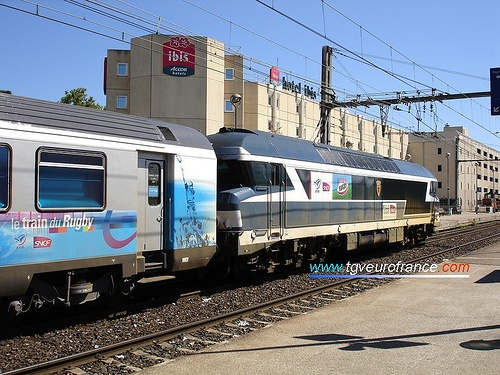
\includegraphics[width=.2\textwidth,height=.15\textwidth]{image/example/2007_004483.jpg}
	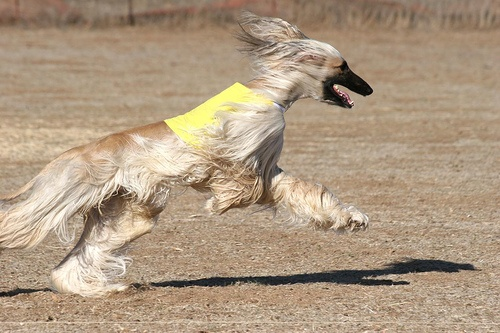
\includegraphics[width=.2\textwidth,height=.15\textwidth]{image/example/2007_003194.jpg}
	\\
	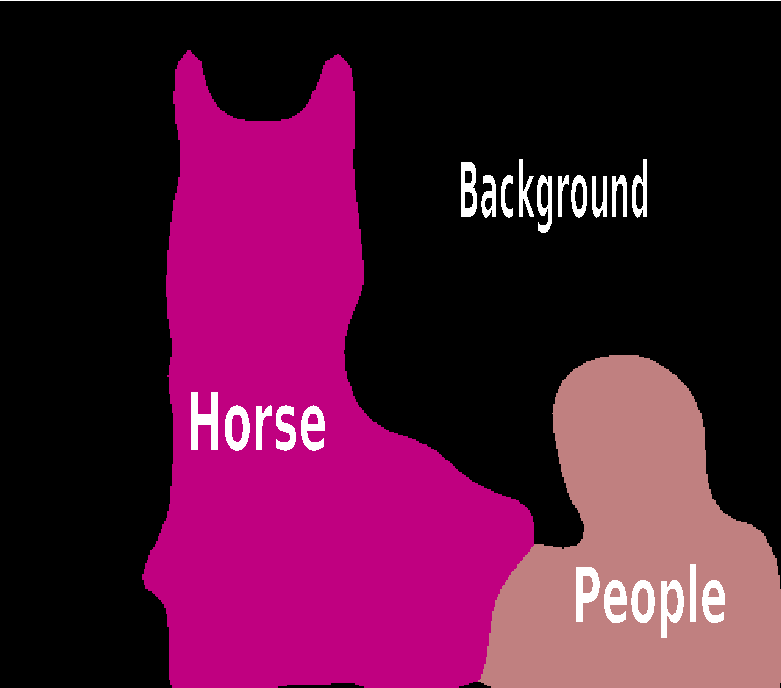
\includegraphics[width=.2\textwidth,height=.15\textwidth]{image/example/2007_000799.pdf}
	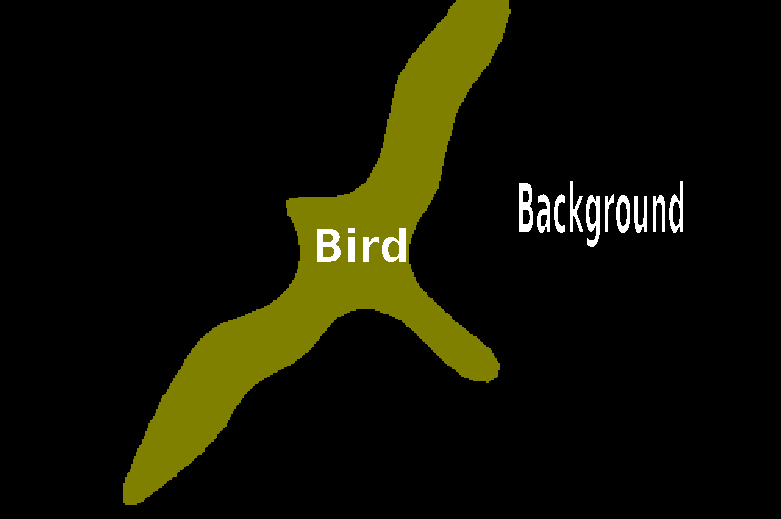
\includegraphics[width=.2\textwidth,height=.15\textwidth]{image/example/2007_002094.pdf}
	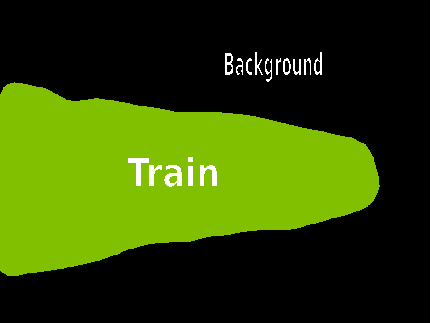
\includegraphics[width=.2\textwidth,height=.15\textwidth]{image/example/2007_004483.pdf}
	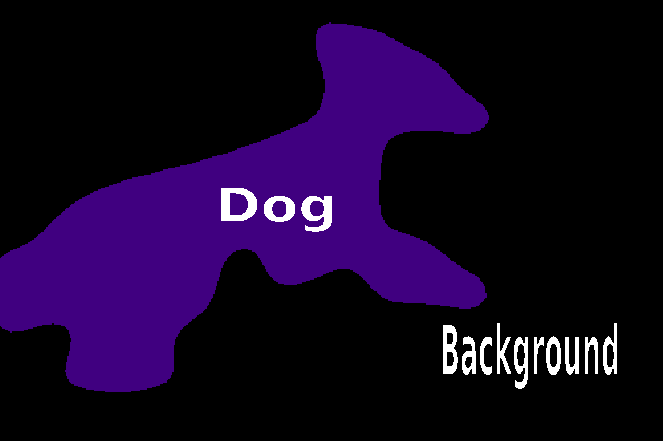
\includegraphics[width=.2\textwidth,height=.15\textwidth]{image/example/2007_003194.pdf}
	\caption{并排的多张图像}
	\label{fig:example1}
\end{figure}
\endinput

% \begin{figure}[h]
\centering
	\makebox[0.11\textwidth]{\scriptsize 图像}
	\enspace
	\makebox[0.11\textwidth]{\scriptsize 真值}
	\enspace
	\makebox[0.11\textwidth]{\scriptsize CNN+5LSTM\textbf{1}}
	\enspace\thinspace
	\makebox[0.11\textwidth]{\scriptsize CNN+5LSTM\textbf{2}}
	\enspace\thinspace
	\makebox[0.11\textwidth]{\scriptsize CNN+5LSTM\textbf{3}}
	\enspace\thinspace
	\makebox[0.11\textwidth]{\scriptsize CNN+5LSTM\textbf{4}}
	\enspace\thinspace
	\makebox[0.11\textwidth]{\scriptsize CNN+5LSTM\textbf{5}}\\
	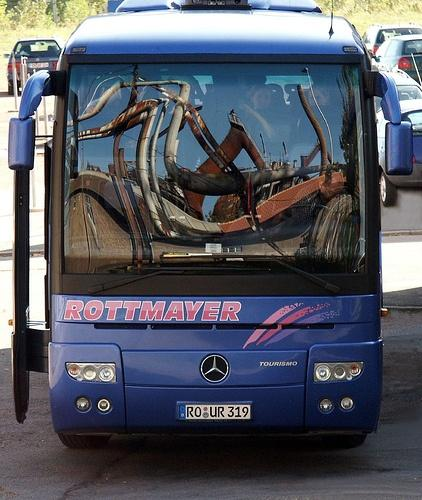
\includegraphics[width=0.11\textwidth]{image/improvement/2007_000663.jpg}
	\enspace\thinspace %\hfill
	
\includegraphics[width=0.11\textwidth]{image/improvement/2007_000663.png}
	\enspace\thinspace
	
\includegraphics[width=0.11\textwidth]{image/improvement/2007_000663_1.png}
	\enspace\thinspace
	
\includegraphics[width=0.11\textwidth]{image/improvement/2007_000663_2.png}
	\enspace\thinspace
	
\includegraphics[width=0.11\textwidth]{image/improvement/2007_000663_3.png}
	\enspace\thinspace
	
\includegraphics[width=0.11\textwidth]{image/improvement/2007_000663_4.png}
	\enspace\thinspace
	
\includegraphics[width=0.11\textwidth]{image/improvement/2007_000663_5.png}
	\enspace\thinspace
	\caption{并排的多张图像加各自的注解}
	\label{fig:improvement}
\end{figure}


% \subsection{两列图像的插入}
% \label{sec:complex}
% \begin{figure}[h!] % image examples & compare
	\begin{subfigure}{0.55\textwidth}
		\makebox[0.18\textwidth]{\scriptsize Grid-5LSTM}
		\makebox[0.18\textwidth]{\scriptsize FCN-8s\cite{long2015fully}}
		\makebox[0.18\textwidth]{\scriptsize SDS\cite{hariharan2014simultaneous}}
		\makebox[0.18\textwidth]{\scriptsize 真值}
		\makebox[0.18\textwidth]{\scriptsize 图像} \\
		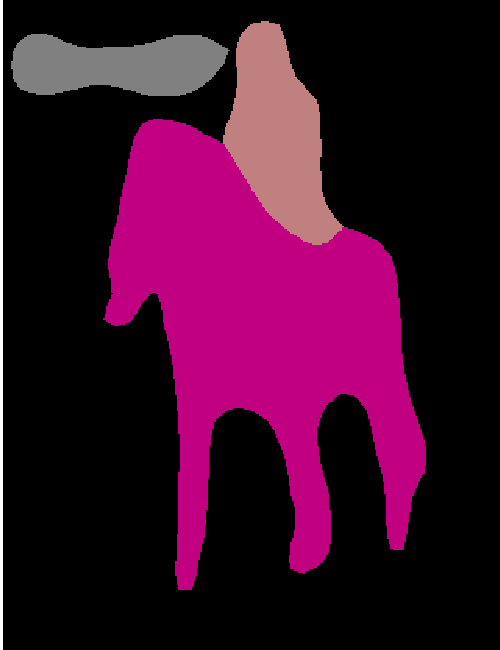
\includegraphics[width=0.18\textwidth]{image/result/compare/my_horse.pdf}
		
\includegraphics[width=0.18\textwidth]{image/result/compare/fcn_horse.png}
		
\includegraphics[width=0.18\textwidth]{image/result/compare/sds_horse.png}
		
\includegraphics[width=0.18\textwidth]{image/result/compare/gt_horse.pdf}
		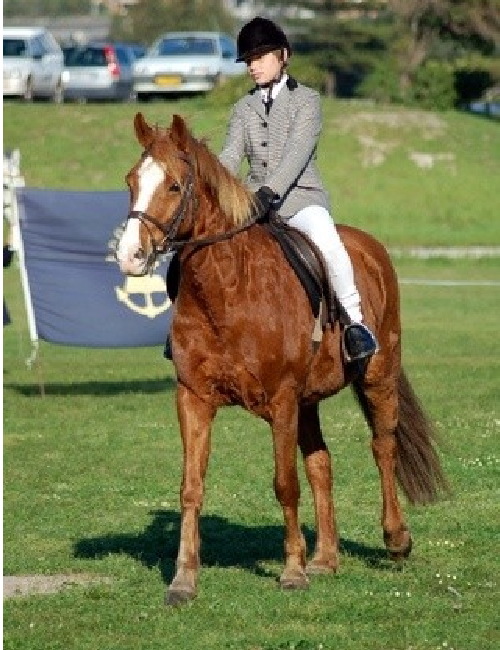
\includegraphics[width=0.18\textwidth]{image/result/compare/im_horse.pdf}
		\\
		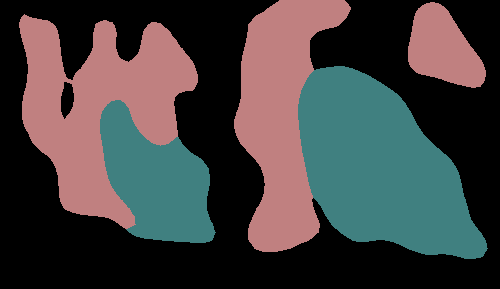
\includegraphics[width=0.18\textwidth]{image/result/compare/my_motor.png}
		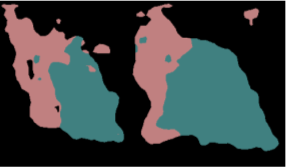
\includegraphics[width=0.18\textwidth]{image/result/compare/fcn_motor.png}
		
\includegraphics[width=0.18\textwidth]{image/result/compare/sds_motor.png}
		
\includegraphics[width=0.18\textwidth]{image/result/compare/2007_005173.png}
		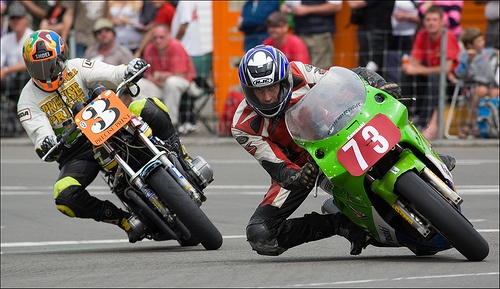
\includegraphics[width=0.18\textwidth]{image/result/compare/2007_005173.jpg}
		\\
		
\includegraphics[width=0.18\textwidth]{image/result/compare/my_sheep.pdf}
		
\includegraphics[width=0.18\textwidth]{image/result/compare/fcn_sheep.png}
		
\includegraphics[width=0.18\textwidth]{image/result/compare/sds_sheep.png}
		
\includegraphics[width=0.18\textwidth]{image/result/compare/gt_sheep.pdf}
		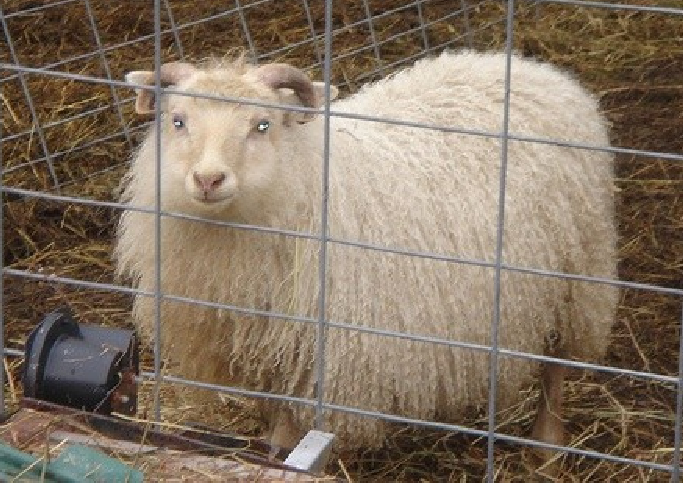
\includegraphics[width=0.18\textwidth]{image/result/compare/im_sheep.pdf}
		\\
		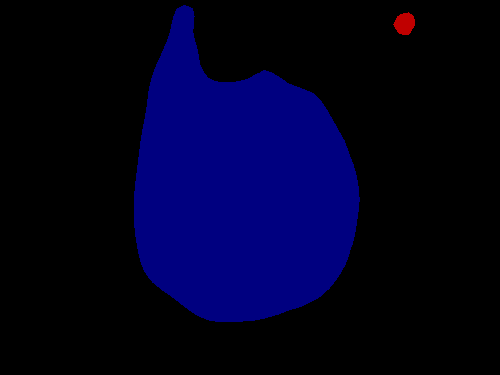
\includegraphics[width=0.18\textwidth]{image/result/compare/my_boat.png}
		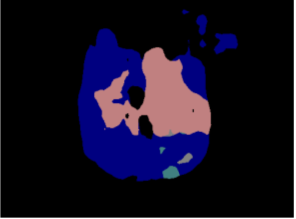
\includegraphics[width=0.18\textwidth]{image/result/compare/fcn_boat.png}
		
\includegraphics[width=0.18\textwidth]{image/result/compare/sds_boat.png}
		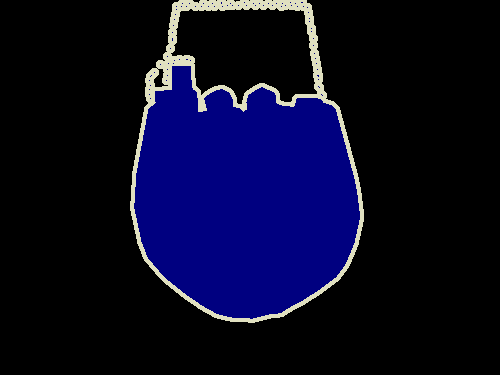
\includegraphics[width=0.18\textwidth]{image/result/compare/2007_004241.png}
		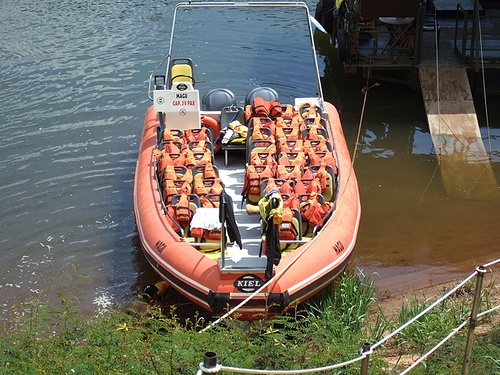
\includegraphics[width=0.18\textwidth]{image/result/compare/2007_004241.jpg}
		\caption{左边的图像}
		\label{fig:compare1}
	\end{subfigure}
	\begin{subfigure}{0.4\textwidth}
		\centering
%		\makebox[0.3\textwidth]{} \\
%		\makebox[0.3\textwidth]{} \\
		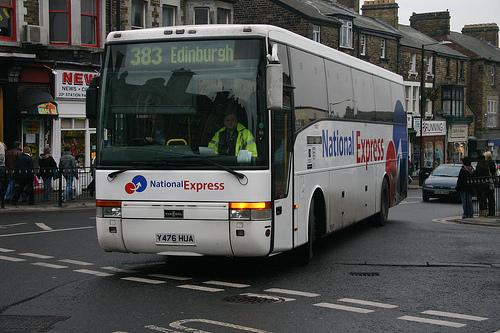
\includegraphics[width=0.25\textwidth]{image/result/compare/2010_005284.jpg}
		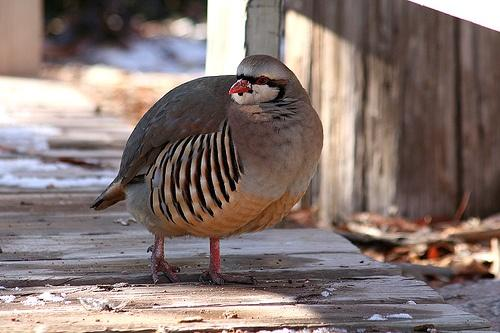
\includegraphics[width=0.25\textwidth]{image/result/compare/2007_003349.jpg}
		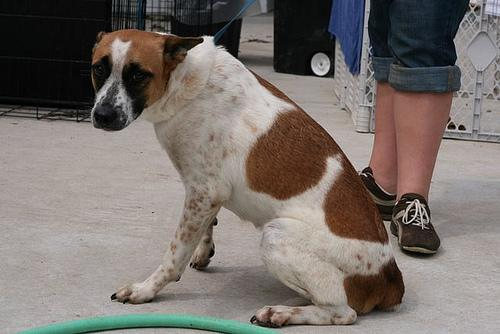
\includegraphics[width=0.25\textwidth]{image/result/compare/2009_004507.jpg} 
		\\
		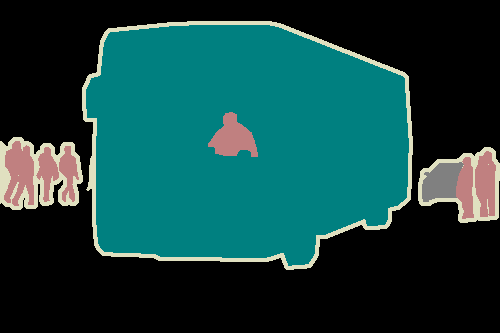
\includegraphics[width=0.25\textwidth]{image/result/compare/2010_005284.png}
		
\includegraphics[width=0.25\textwidth]{image/result/compare/2007_003349.png}
		
\includegraphics[width=0.25\textwidth]{image/result/compare/2009_004507.png} \\
		
\includegraphics[width=0.25\textwidth]{image/result/compare/zoom_bus.png}
		
\includegraphics[width=0.25\textwidth]{image/result/compare/zoom_bird.png}
		
\includegraphics[width=0.25\textwidth]{image/result/compare/zoom_dog.png} \\
		
\includegraphics[width=0.25\textwidth]{image/result/compare/deeplab_bus.png}
		
\includegraphics[width=0.25\textwidth]{image/result/compare/deeplab_bird.png}
		\includegraphics[width=0.25\textwidth]{image/result/compare/deeplab_dog.png} \\
		\includegraphics[width=0.25\textwidth]{image/result/compare/my_bus.png}
		\includegraphics[width=0.25\textwidth]{image/result/compare/my_bird.png}
		\includegraphics[width=0.25\textwidth]{image/result/compare/my_dog.png} 
		\caption{右边的图像}
		\label{fig:compare2}
	\end{subfigure}
	\caption{复杂的两列对象的插入}
	\label{fig:complex}
\end{figure}


% \subsection{矢量图像的插入}
% \label{sec:vec_fig}
% 这是几个使用pgfplots画的矢量图像\footnote{\url{\url{https://www.sharelatex.com/learn/Pgfplots\_package}}},pgfplots包还能画出更加炫酷的图像。
% \begin{figure}[h]
	\centering
	\begin{tikzpicture}
	\begin{axis}[
	    x tick label style={
			/pgf/number format/1000 sep=},
		ylabel=评论数量,
		xlabel=评论长度($\times$5),
		enlargelimits=0.05,
		legend style={at={(0.5,-0.2)},
		anchor=north,legend columns=-1},
		ybar interval=.7,
	]
	\addplot 
		coordinates {(1, 14455) (2, 28483) (3, 27614) (4, 24472) (5, 20409) (6, 16657) (7, 13373) (8, 10948) (9, 8557) (10, 6994) (11, 5601) (12, 4665) (13, 2279) (14, 22796)};
	\addplot 
		coordinates {(1, 1445) (2, 8483) (3, 2614) (4, 2472) (5, 2009) (6, 1657) (7, 1373) (8, 1948) (9, 557) (10, 994) (11, 501) (12, 466) (13, 22967) (14, 2276)};
	\legend{图例1, 图例2}
	\end{axis}
	\end{tikzpicture}
	\caption{使用pgfplots画的矢量图像}
 	\label{fig:statistiss}
\end{figure}




% 关于图,详细来说

% 1、插图应与文字内容相符,技术内容正确。所有制图应符合国家标准和专业标准。对无规定符号的图形应采用该行业的常用画法。

% 2、每幅插图应有标题和序号,全文的插图可以统一编序,也可以逐章单独编序。采取哪一种方式应和表格、公式的编序方式统一。图序必须连续,不重复,不跳缺。
% 3、由若干分图组成的插图,分图用a、b、c……标序。分图的图名以及图中各种代号的意义,以图注形式写在图题下方,先写分图名,另起行写代号的意义。

% 4、图与图标题、图序号为一个整体,不得拆开排版为两页。当页空白不够排版该图整体时,可将其后文字部分提前,将图移至次页最前面。

% 5、对坐标轴必须进行文字标示,有数字标注的坐标图必须注明坐标单位

% \clearpage



% \section{表格的插入}
% \label{sec:tables}
% \begin{table}[h] %voc table result
	\centering
		\begin{tabular}{*{4}{c}}
			\toprule
	 		Method & Pixel Acc. & Mean Acc. & Mean Iu.\\
			\midrule
			Liu等人\cite{liu2011sift}  & 76.7 & - & -\\
		Tighe等人\cite{tighe2013finding}  & 78.6 & 39.2 & -\\
			FCN-16s\cite{long2015fully} & 85.2 & \textbf{51.7} & 39.5\\
			Deeplab-LargeFOV\cite{chen14semantic} & 85.6 & 51.2 & 39.7\\
			\midrule
			Grid-LSTM5 & \textbf{86.2} & 51.0 & \textbf{41.2}\\
			\bottomrule
		\end{tabular}
		\caption{典型的实验对比表格}		
		\label{tab:siftflow}
\end{table}

% \begin{table}[h] %voc table result
\centering
	\resizebox{\textwidth}{!}{
	\begin{tabular}{c|*{20}{c}|c}
		\toprule
		Method & aero & bike & bird & boat & bottle & bus & car & cat & chair & cow & table & dog & horse & mbike & person & plant & shep & sofa & train & tv & mIoU.\\
		\midrule
		CNN				   & 72.6 & 29.6 & 70.2 & 53.1 & 65.1 & 81.0 & 74.3 & 79.8 & 25.0 & 64.8 & 47.8 & 69.5 & 66.2 & 65.2 & 74.2 & 42.1 & 69.6 & 38.8 & 74.4 & 58.6 & 62.5\\
		CNN+\textbf{1}LSTM & 71.5 & 30.6 & 70.5 & 53.8 & 64.9 & 82.4 & 77.1 & 79.5 & 25.1 & 65.8 & 47.8 & 71.5 & 64.6 & 67.0 & 74.0 & 43.9 & 69.6 & 38.6 & 74.9 & 59.4 & 63.0\\
		CNN+\textbf{2}LSTM & 76.1 & 32.6 & 72.1 & 57.0 & 65.3 & 83.6 & 75.4 & 81.7 & 24.7 & 69.3 & 47.5 & 72.3 & 68.9 & 69.5 & 74.7 & 41.5 & 69.8 & 38.3 & 77.8 & 62.1 & 64.3 \\
		CNN+\textbf{3}LSTM & 77.7 & 32.3 & 72.6 & 60.0 & 68.3 & 85.5 & 78.5 & 82.3 & 25.3 & 71.1 & 49.7 & 71.5 & 69.7 & 70.8 & 75.9 & 47.9 & 71.2 & 38.9 & 80.2 & 61.7 & 65.8 \\
		CNN+\textbf{4}LSTM & 79.1 & \textbf{33.7} & \textbf{73.6} & \textbf{62.0} & \textbf{70.4} & 85.5 & \textbf{80.9} & 83.7 & \textbf{24.1} & 70.7 & 45.7 & 73.7 & 69.6 & 72.1 & 75.6 & 47.2 & \textbf{76.0} & 37.3 & 80.5 & 62.2 & 66.4 \\
		CNN+\textbf{5}LSTM & \textbf{79.9} & 33.6 & \textbf{73.6} & 61.7 & 68.0 & \textbf{88.5} & \textbf{80.9} & \textbf{84.0} & 23.6 & \textbf{71.3} & \textbf{49.7} & \textbf{73.1} & \textbf{71.3} & \textbf{72.9} & \textbf{76.4} & \textbf{48.9} & 75.1 & \textbf{38.1} & \textbf{84.5} & \textbf{63.8} & \textbf{67.2} \\
		\midrule
		CNN+\textbf{5}LSTM$^\dag$ & 84.8 & 36.4 & 82.0 & 69.4 & 73.0 & 87.2 & 81.8 & 86.1 & 34.5 & 82.4 & 53.1 & 81.5 & 77.4 & 79.0 & 81.3 & 54.8 & 81.1 & 47.0 & 84.3 & 67.3 & 72.3 \\
		\bottomrule
	\end{tabular}}
	\caption{复杂一些的表格}		
	\label{tab:vocval}
\end{table}


% \section{公式}
% \label{sec:formula}
% 没有编号的公式
% \begin{align*}
% \begin{split}
% 	\label{eq:feedforward}
% 	\mybold{z}^{(l)} & = \mybold{W}^{(l)}\mybold{a}^{(l-1)} + \mybold{b}^{(l)} \\
% 	\mybold{a}^{(l)} & = f(\mybold{z}^{(l)})
% \end{split}
% \end{align*}
% 公式中含有中文
% \begin{align}
% 	\begin{split}
% 	\mbox{像素准确率} &= \sum_{i=1}^{n_{cl}}n_{ii} / \sum_{i=1}^{n_{cl}}t_i \\
% 		\mbox{平均像素准确率} &= \frac{1}{n_{cl}} \sum_{i=1}^{n_{cl}}(n_{ii}/ t_i) \\
% 	\mbox{Mean IU} &= \frac{1}{n_{cl}} \sum_{i=1}^{n_{cl}}\frac{n_{ii}}{t_i + \sum_j^{n_{cl}} n_{ji} - n_{ii}}
% 	\end{split}
% \end{align}
% 公式中含有矩阵
% \begin{equation}
% 	\textbf{H} = \begin{bmatrix}
% 		I*\mybold{x}_i \\ \textbf{h}
% 	\end{bmatrix}
% \end{equation}
% 每行后面都有编号的公式
% \begin{align}
% 	\frac{\partial}{\partial W_{ij}^{(l)}} J(\mybold{W},\mybold{b};\mybold{x},y) &= \frac{\partial J(\mybold{W},\mybold{b};\mybold{x},y)}{\partial z_i^{(l+1)}}\cdot \frac{\partial z_i^{(l+1)}}{\partial W_{ij}^{(l)}} = \delta_i^{(l+1)}a_j^{(l)} \\
% 	\frac{\partial}{\partial b_i^{(l)}} J(\mybold{W},\mybold{b};\mybold{x},y) &= \frac{\partial J(\mybold{W},\mybold{b};\mybold{x},y)}{\partial z_i^{(l+1)}}\cdot \frac{\partial z_i^{(l+1)}}{\partial b_i^{(l)}} = \delta_i^{(l+1)}
% \end{align}

% \section{算法流程图}
% \label{sec:algorithm}
% \begin{algorithm}[h]
% \KwIn{$m$个训练样本}
% \lFor{$l=1$ \emph{\KwTo} $n_l$}{
% 初始化:$\Delta \mybold{W}^{(l)}=0$,$\Delta \mybold{b}^{(l)}=0$}
% \ForEach{训练样本}{
% 	\lFor{$l=1$ \emph{\KwTo} $n_l-1$}{
% 	前向传播:$\mybold{z}^{(l+1)}=\mybold{W}^la^l+\mybold{b}^l$,$\mybold{a}^{(l+1)}=f(\mybold{z}^{(l+1)})$}
% 	输出误差计算:$\delta^{(n_l)} = \frac{\partial}{\partial \mybold{z}^{(n_l)}} J(\mybold{W},\mybold{b};\mybold{x},y)$\;
% 	\lFor{$l=n_l-1$ \emph{\KwTo} $1$}{
% 	后向传播:$\delta^{(l)} = \bigl((\mybold{W}^{(l)})^T \delta^{(l+1)}\bigr)f'(\mybold{z}^{(l)})$}
% 	\ForAll{层l}{
% 		计算梯度:$\nabla_{\mybold{W}^{(l)}}J(\mybold{W},\mybold{b};\mybold{x},y)=\delta^{(l+1)}(\mybold{a}^{(l)})^T$ \\
% 		\hspace{60pt}$\nabla_{\mybold{b}^{(l)}}J(\mybold{W},\mybold{b};\mybold{x},y)=\delta^{(l+1)}$\;
% 		累加梯度:$\Delta \mybold{W}^{(l)} \leftarrow \Delta \mybold{W}^{(l)} + \nabla_{\mybold{W}^{(l)}}J(\mybold{W},\mybold{b};\mybold{x},y)$; \\
% 		\hspace{60pt}$\Delta \mybold{b}^{(l)} \leftarrow \Delta \mybold{b}^{(l)} + \nabla_{\mybold{b}^{(l)}}J(\mybold{W},\mybold{b};\mybold{x},y)$\;
% 	}
% }
% \ForAll{层$l$}{
% 	更新权重:$\mybold{W}^{(l)} \leftarrow \mybold{W}^{(l)} - \alpha \biggl[\frac 1m \Delta \mybold{W}^{(l)}]$ \\
% 	\hspace{60pt} $\mybold{b}^{(l)} \leftarrow \mybold{b}^{(l)} - \alpha \biggl[\frac 1m \Delta \mybold{b}^{(l)}\biggr]$
% }
% \caption{梯度下降算法}
% \label{algo:sgd}
% \end{algorithm}

% \section{例子与证明}
% \subsection{例子}
% \begin{eg}
%   这是一个例子, 用以验证特殊环境的字体成功更改为楷体.
% \end{eg}

% \begin{proof}
%   1. 大前提
%   2. 小前提
%   结论: 示例结论
% \end{proof}

% \section{其他的一些用法}
% \label{sec:font}
% \subsection{子章节编号}
% \label{sec:font:subsection}
% \subsubsection{更小的章节}
% \label{sec:font:subsection:subsub}
% 更小的章节编号也是支持的。

% \subsection{列表的使用}
% \label{sec:font:list}

% 这是一个无序列表
% \begin{itemize}
% 	\item 引用文献\cite{long2015fully}
% 	\item 字体{\color{red}{变红}},\textbf{粗体}
% \end{itemize}

% 这是一个有序列表
% \begin{enumerate}
% 	\item 索引前面的章节 \ref{sec:formula}、图像\ref{fig:complex}、表格\ref{tab:siftflow}
% 	\item 加脚注\footnote{http://cs231n.github.io/transfer-learning/}
% \end{enumerate}


